

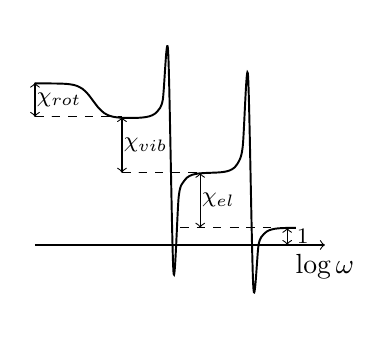
\begin{tikzpicture}[
declare function={ 
epsr(\w,\wr,\g) = (\wr^2-\w^2)/((\wr^2-\w^2)^2+\g^2*\w^2);
alles(\w) = 1 + 2e2* (epsr(\w,1e1,1e2) + 4e3 * epsr(\w,5e2,1e2) +   1e9 * epsr(\w,25e4,5e4));
  }
]
%\useasboundingbox (0,0) rectangle (5,5);
%\draw (0,0) rectangle (5,5);

\begin{axis}[no markers,
 samples=50, smooth,
     %     ymin=-0.3, ymax=1,
       axis y line=none,
          axis x line=none,
        xmode=log,
           width= 6cm]
           
\addplot [domain=1e-2:1e7,  line width=0.7pt]  
{ alles(x) };

\addplot[->] coordinates   {(1e-2,0) (1e8, 0)};
\node  [anchor= north] at (axis cs: 1e8,0) {$\log \omega$} ;

\addplot[dashed] coordinates   {(1e3,1) (1e7, 1)};
\addplot[dashed] coordinates   {(1e1,4.2) (1e4, 4.2)};
\addplot[dashed] coordinates   {(1e-2,7.45) (1e1, 7.45)};

\addplot[<->] coordinates   {(5e6,0) (5e6, 1)};
\node  [anchor= west] at (axis cs: 5e6,0.5) {\footnotesize $1$} ;

\addplot[<->] coordinates   {(5e3,1) (5e3, 4.2)};
\node  [anchor= west,xshift=-1mm] at (axis cs: 5e3,2.6) {\footnotesize $\chi_{el}$} ;

\addplot[<->] coordinates   {(1e1,7.45) (1e1, 4.2)};
\node  [anchor= west,xshift=-1mm] at (axis cs: 1e1,5.8) {\footnotesize $\chi_{vib}$} ;

\addplot[<->] coordinates   {(1e-2,7.45) (1e-2, 9.45)};
\node  [anchor= west, xshift=-1mm] at (axis cs: 1e-2,8.45) {\footnotesize $\chi_{rot}$} ;


%\node (w0) [anchor= north ] at (axis cs: 99,-0.002) {$\omega_0$} ;
%\draw[->] (w0) -- (axis cs: 100,0);
%
%
%\node [anchor= north] at (axis cs: 94.5,0.007) {$\epsilon' -1 $} ;
%\node [anchor= north] at (axis cs: 101.5,0.02) {$\epsilon'' $} ;

%
\end{axis}

\end{tikzpicture}
